\documentclass[10pt,dvipsnames,enabledeprecatedfontcommands]{scrartcl}
\usepackage{lmodern}
\usepackage{amssymb,amsmath}
\usepackage{ifxetex,ifluatex}
\usepackage{fixltx2e} % provides \textsubscript
\ifnum 0\ifxetex 1\fi\ifluatex 1\fi=0 % if pdftex
  \usepackage[T1]{fontenc}
  \usepackage[utf8]{inputenc}
\else % if luatex or xelatex
  \ifxetex
    \usepackage{mathspec}
  \else
    \usepackage{fontspec}
  \fi
  \defaultfontfeatures{Ligatures=TeX,Scale=MatchLowercase}
\fi
% use upquote if available, for straight quotes in verbatim environments
\IfFileExists{upquote.sty}{\usepackage{upquote}}{}
% use microtype if available
\IfFileExists{microtype.sty}{%
\usepackage[]{microtype}
\UseMicrotypeSet[protrusion]{basicmath} % disable protrusion for tt fonts
}{}
\PassOptionsToPackage{hyphens}{url} % url is loaded by hyperref
\usepackage[unicode=true]{hyperref}
\PassOptionsToPackage{usenames,dvipsnames}{color} % color is loaded by hyperref
\hypersetup{
            pdftitle={A bayesian method of cosine-based word2vec bias},
            pdfauthor={Alicja Dobrzeniecka and Rafal Urbaniak},
            colorlinks=true,
            linkcolor=Maroon,
            citecolor=Blue,
            urlcolor=blue,
            breaklinks=true}
\urlstyle{same}  % don't use monospace font for urls
\usepackage{color}
\usepackage{fancyvrb}
\newcommand{\VerbBar}{|}
\newcommand{\VERB}{\Verb[commandchars=\\\{\}]}
\DefineVerbatimEnvironment{Highlighting}{Verbatim}{commandchars=\\\{\}}
% Add ',fontsize=\small' for more characters per line
\usepackage{framed}
\definecolor{shadecolor}{RGB}{248,248,248}
\newenvironment{Shaded}{\begin{snugshade}}{\end{snugshade}}
\newcommand{\KeywordTok}[1]{\textcolor[rgb]{0.13,0.29,0.53}{\textbf{#1}}}
\newcommand{\DataTypeTok}[1]{\textcolor[rgb]{0.13,0.29,0.53}{#1}}
\newcommand{\DecValTok}[1]{\textcolor[rgb]{0.00,0.00,0.81}{#1}}
\newcommand{\BaseNTok}[1]{\textcolor[rgb]{0.00,0.00,0.81}{#1}}
\newcommand{\FloatTok}[1]{\textcolor[rgb]{0.00,0.00,0.81}{#1}}
\newcommand{\ConstantTok}[1]{\textcolor[rgb]{0.00,0.00,0.00}{#1}}
\newcommand{\CharTok}[1]{\textcolor[rgb]{0.31,0.60,0.02}{#1}}
\newcommand{\SpecialCharTok}[1]{\textcolor[rgb]{0.00,0.00,0.00}{#1}}
\newcommand{\StringTok}[1]{\textcolor[rgb]{0.31,0.60,0.02}{#1}}
\newcommand{\VerbatimStringTok}[1]{\textcolor[rgb]{0.31,0.60,0.02}{#1}}
\newcommand{\SpecialStringTok}[1]{\textcolor[rgb]{0.31,0.60,0.02}{#1}}
\newcommand{\ImportTok}[1]{#1}
\newcommand{\CommentTok}[1]{\textcolor[rgb]{0.56,0.35,0.01}{\textit{#1}}}
\newcommand{\DocumentationTok}[1]{\textcolor[rgb]{0.56,0.35,0.01}{\textbf{\textit{#1}}}}
\newcommand{\AnnotationTok}[1]{\textcolor[rgb]{0.56,0.35,0.01}{\textbf{\textit{#1}}}}
\newcommand{\CommentVarTok}[1]{\textcolor[rgb]{0.56,0.35,0.01}{\textbf{\textit{#1}}}}
\newcommand{\OtherTok}[1]{\textcolor[rgb]{0.56,0.35,0.01}{#1}}
\newcommand{\FunctionTok}[1]{\textcolor[rgb]{0.00,0.00,0.00}{#1}}
\newcommand{\VariableTok}[1]{\textcolor[rgb]{0.00,0.00,0.00}{#1}}
\newcommand{\ControlFlowTok}[1]{\textcolor[rgb]{0.13,0.29,0.53}{\textbf{#1}}}
\newcommand{\OperatorTok}[1]{\textcolor[rgb]{0.81,0.36,0.00}{\textbf{#1}}}
\newcommand{\BuiltInTok}[1]{#1}
\newcommand{\ExtensionTok}[1]{#1}
\newcommand{\PreprocessorTok}[1]{\textcolor[rgb]{0.56,0.35,0.01}{\textit{#1}}}
\newcommand{\AttributeTok}[1]{\textcolor[rgb]{0.77,0.63,0.00}{#1}}
\newcommand{\RegionMarkerTok}[1]{#1}
\newcommand{\InformationTok}[1]{\textcolor[rgb]{0.56,0.35,0.01}{\textbf{\textit{#1}}}}
\newcommand{\WarningTok}[1]{\textcolor[rgb]{0.56,0.35,0.01}{\textbf{\textit{#1}}}}
\newcommand{\AlertTok}[1]{\textcolor[rgb]{0.94,0.16,0.16}{#1}}
\newcommand{\ErrorTok}[1]{\textcolor[rgb]{0.64,0.00,0.00}{\textbf{#1}}}
\newcommand{\NormalTok}[1]{#1}
\usepackage{graphicx,grffile}
\makeatletter
\def\maxwidth{\ifdim\Gin@nat@width>\linewidth\linewidth\else\Gin@nat@width\fi}
\def\maxheight{\ifdim\Gin@nat@height>\textheight\textheight\else\Gin@nat@height\fi}
\makeatother
% Scale images if necessary, so that they will not overflow the page
% margins by default, and it is still possible to overwrite the defaults
% using explicit options in \includegraphics[width, height, ...]{}
\setkeys{Gin}{width=\maxwidth,height=\maxheight,keepaspectratio}
\IfFileExists{parskip.sty}{%
\usepackage{parskip}
}{% else
\setlength{\parindent}{0pt}
\setlength{\parskip}{6pt plus 2pt minus 1pt}
}
\setlength{\emergencystretch}{3em}  % prevent overfull lines
\providecommand{\tightlist}{%
  \setlength{\itemsep}{0pt}\setlength{\parskip}{0pt}}
\setcounter{secnumdepth}{5}
% Redefines (sub)paragraphs to behave more like sections
\ifx\paragraph\undefined\else
\let\oldparagraph\paragraph
\renewcommand{\paragraph}[1]{\oldparagraph{#1}\mbox{}}
\fi
\ifx\subparagraph\undefined\else
\let\oldsubparagraph\subparagraph
\renewcommand{\subparagraph}[1]{\oldsubparagraph{#1}\mbox{}}
\fi

% set default figure placement to htbp
\makeatletter
\def\fps@figure{htbp}
\makeatother

%\documentclass{article}

% %packages
 \usepackage{booktabs}

\usepackage{multirow}

\usepackage{graphicx}
\usepackage{longtable}
\usepackage{ragged2e}
\usepackage{etex}
%\usepackage{yfonts}
\usepackage{marvosym}
\usepackage[notextcomp]{kpfonts}
\usepackage{nicefrac}
\newcommand*{\QED}{\hfill \footnotesize {\sc Q.e.d.}}
\usepackage{floatrow}

\usepackage[textsize=footnotesize]{todonotes}
%\linespread{1.5}


\setlength{\parindent}{10pt}
\setlength{\parskip}{1pt}


%language
\usepackage{times}
\usepackage{t1enc}
%\usepackage[utf8x]{inputenc}
%\usepackage[polish]{babel}
%\usepackage{polski}

\usepackage{mathptmx}
\usepackage[scaled=0.88]{helvet}


%AMS
\usepackage{amsfonts}
\usepackage{amssymb}
\usepackage{amsthm}
\usepackage{amsmath}
\usepackage{mathtools}

\usepackage{geometry}
 \geometry{a4paper,left=35mm,top=20mm,}


%environments
\newtheorem{fact}{Fact}



%abbreviations
\newcommand{\ra}{\rangle}
\newcommand{\la}{\langle}
\newcommand{\n}{\neg}
\newcommand{\et}{\wedge}
\newcommand{\jt}{\rightarrow}
\newcommand{\ko}[1]{\forall  #1\,}
\newcommand{\ro}{\leftrightarrow}
\newcommand{\exi}[1]{\exists\, {_{#1}}}
\newcommand{\pr}[1]{\mathsf{P}(#1)}
\newcommand{\cost}{\mathsf{cost}}


\newcommand{\odds}{\mathsf{Odds}}
\newcommand{\ind}{\mathsf{Ind}}
\newcommand{\nf}[2]{\nicefrac{#1\,}{#2}}
\newcommand{\R}[1]{\texttt{#1}}
\newcommand{\prr}[1]{\mbox{$\mathtt{P}_{prior}(#1)$}}
\newcommand{\prp}[1]{\mbox{$\mathtt{P}_{posterior}(#1)$}}



\newtheorem{q}{\color{blue}Question}
\newtheorem{lemma}{Lemma}
\newtheorem{theorem}{Theorem}



%technical intermezzo
%---------------------

\newcommand{\intermezzoa}{
	\begin{minipage}[c]{13cm}
	\begin{center}\rule{10cm}{0.4pt}



	\tiny{\sc Optional Content Starts}
	
	\vspace{-1mm}
	
	\rule{10cm}{0.4pt}\end{center}
	\end{minipage}\nopagebreak 
	}


\newcommand{\intermezzob}{\nopagebreak 
	\begin{minipage}[c]{13cm}
	\begin{center}\rule{10cm}{0.4pt}

	\tiny{\sc Optional Content Ends}
	
	\vspace{-1mm}
	
	\rule{10cm}{0.4pt}\end{center}
	\end{minipage}
	}
%--------------------






















\newtheorem*{reply*}{Reply}
\usepackage{enumitem}
\newcommand{\question}[1]{\begin{enumerate}[resume,leftmargin=0cm,labelsep=0cm,align=left]
\item #1
\end{enumerate}}

\usepackage{float}

% \setbeamertemplate{blocks}[rounded][shadow=true]
% \setbeamertemplate{itemize items}[ball]
% \AtBeginPart{}
% \AtBeginSection{}
% \AtBeginSubsection{}
% \AtBeginSubsubsection{}
% \setlength{\emergencystretch}{0em}
% \setlength{\parskip}{0pt}






\usepackage[authoryear]{natbib}

%\bibliographystyle{apalike}

\title{A bayesian method of cosine-based word2vec bias}
\author{Alicja Dobrzeniecka and Rafal Urbaniak}
\date{}

\begin{document}
\maketitle

\tableofcontents

\section{Cosine-based measures of
bias}\label{cosine-based-measures-of-bias}

\todo{two introductory}

One of the first measures in the discussion has been developed by
Bolukbasi, Chang, Zou, Saligrama, \& Kalai (2016). There, the gender
bias of a word \(w\) is understood as its projection on the gender
direction \(\vec{w} \cdot (\overrightarrow{he} - \overrightarrow{she})\)
(the gender direction is the top principal compontent of ten gender pair
difference vectors). The underlying idea is that no bias is present if
non-explicitly gendered words are in equal distance to both elements in
all explicitly gender pairs. Given the (ideally) gender neutral words
\(N\) and the gender direction \(g\) the direct direct gender bias is
defined as the average distance of the words in \(N\) from \(g\) (\(c\)
is a parameter determining how strict we want to be):

\begin{align}
\mathsf{directBias_c(N,g)} & = \frac{\sum_{w\in N}\vert \mathsf{cos}(\vec{w},g)\vert^c}{\vert N \vert }
\end{align}

The use of projections has been ciriticized for instance by Gonen \&
Goldberg (2019), who point out that while gender-direction might be an
indicator of bias, it is only one possible manifestation of it, and
reducing a projection of words might be insufficient. For instance,
``math'' and ``delicate'' might be in equal distance to both explicitly
gendered words while being closer to quite different stereotypical
attribute words. Further, the authors point out that most word pairs
preserve similarity under debiasing meant to minimize projection-based
bias.\footnote{Bolukbasi et al. (2016) use also another method which
  involves analogies and their evaluations by human users on Mechanical
  Turk. It is discussed and criticized in (Nissim, Noord, \& Goot,
  2020).}

To measure bias in word embeddings, Caliskan, Bryson, \& Narayanan
(2017) proposed the Word Embedding Association Test (WEAT). The idea is
that the measure of biases between two sets of target words, \(X\) and
\(Y\), (we call them protected words) should be quantified in terms of
the cosine similarity between the protected words and attribute words
coming from two sets of stereotype attribute words, \(A\) and \(B\)
(we'll call them attributes). For instance, \(X\) might be a set of male
names, \(Y\) a set of female names, \(A\) might contain stereotypically
male-related career words, and \(B\) stereotypically female-related
family words. WEAT is a modification of the Implicit Association Test
(IAT) (Nosek, Banaji, \& Greenwald, 2002) used in psychology and uses
almost the same word sets, allowing for a \emph{prima facie} sensible
comparison with bias in humans. If the person's attitude towards given
pair of concept is to be interpreted as neutral, there should be no
noticeable task completion time difference, and the final value from the
formula should be around 0. Let \(f\) be a similarity measure (usually,
cosine similarity). The association difference for a term \(t\) is:

\begin{align}
s(t,A,B) & = \frac{\sum_{a\in A}f(t,a)}{\vert A\vert} - \frac{\sum_{b\in B}f(t,b)}{\vert B\vert}
\end{align}

\noindent then, the association difference between \(A\) a \(B\) is:

\begin{align}
s(X,Y,A,B) & = \sum_{x\in X} s(x,A,B) -  \sum_{y\in Y} s(y,A,B)
\end{align}

\noindent
\(s(X,Y,A,B)\) is the statistic used in the signifcance test, and the
\(p\)-value obtained by bootstrapping: it is the frequency of
\(s(X_i,Y_i,A,B)>s(X,Y,A,B)\) for all equally sized partitions
\(X_i, Y_i\) of \(X\cup Y\). The effect size is computed by normalizing
the difference in means as follows:

\begin{align}
bias(A,B) & = \frac{
\mu(\{s(x,A,B)\}_{x\in X}) -\mu(\{s(y,A,B)\}_{y\in Y}) 
}{
\sigma(\{s(w,A,B)\}_{w\in X\cup Y})
}
\end{align}

Caliskan et al. (2017) show that significant biases---thus measured---
similar to the ones discovered by IAT can be discovered in word
embeddings. Lauscher \& Glavas (2019) extended the methodology to a
multilingual and cross-lingual setting, arguing that using Euclidean
distance instead of similarity does not make much difference, while the
bias effects vary greatly across embedding models (interestingly, with
social media-text trained embeddings being less biased than those based
on Wikipedia).

A similar methodology is employed by Garg, Schiebinger, Jurafsky, \& Zou
(2018), who employ word embeddings trained on corpora from different
decades to study the shifts in various biases. For instance, to compute
the occupational embeddings bias for women the authors first compute the
average vector of vector emeddings of words that represent women (e.g.
``she'', ``female''), then calculate the Euclidean distance between this
mean vector and words for occupations. Then they take the mean of these
distances and subtract from it the analogously obtained mean for the
average vector of vector embeddings of words that represent men.
Formally they take the relative norm distance between \(X\) and \(Y\) to
be:

\begin{align}
\textsf{relative norm distance} & = \sum_{v_m\in M} \vert \vert v_m - v_X\vert \vert_2 - \vert v_m - v_Y\vert \vert_2
\end{align}

\noindent where the norm used is Euclidean, and \(v_X\) and \(x_Y\) are
average vectors for sets \(X\) and \(Y\) respectively.

({\textbf{???}}) modify WEAT to a multi-class setting, introducing Mean
Average Cosine similarity as a measure of bias (in fact, in the paper
they report distances rather than similarities). Let
\(T = \{t_1, \dots, t_k\}\) be a class of protected word embeddings, and
let each \(A_j\in A\) be a set of attributes stereotypically associated
with a protected word). Then:

\begin{align}
S(t_i, A_j) & = \frac{1}{\vert A_j\vert}\sum_{a\in A_j}\mathsf{cos}(t,a) \\
MAC(T,A) & = \frac{1}{\vert T \vert \,\vert A\vert}\sum_{t_i \in T }\sum_{A_j \in A} S(t_i,A_j)
\end{align}

That is, for each protected word \$T and each attribute class, they
first take the mean for this protected word and all attributes in a
given attribute class, and then take the mean of thus obtained means for
all the protected words. The t-tests they employ are run on average
cosines used to calculate MAC.

\section{Some methodological
problems}\label{some-methodological-problems}

\section{The problem with means of
means}\label{the-problem-with-means-of-means}

The measures described all calculate means of means and their authors
run statistical tests on sets of means. This, however, is problematic
for two related reasons. One, by pre-averaging data we throw away
information about sample sizes. For the former point, think about
proportions: 10 out of 20 and 2 out of 4 give the same mean, but you
would obtain more information by making the former observation rather
than by making the latter. Two, when we pre-average, we remove
variation, and so pre-averaging tend to manufacture false confidence. We
will have more to say about whether this happens in the case of
applications of MAC, for now let's go over a simple example to make the
conceptual point clear.

To illustrate let's employ the formulas used by Caliskan et al. (2017)
in a simple example. Conceptually, all such tests come up with rather
short lists of protected words and rather short lists of stereotypical
attributes. Clearly, these are not complete list. So let's treat them as
samples from richer pools of stereotypical predicates and let's take the
uncertainty and variation involved seriously.

Consider a simple situation in which there are two protected classes,
\(X=\{t_1,t_2\}\) and \(Y=\{t_3,t_4\}\) and two five-element attribute
sets \(A\) and \(B\).

First, we play around with a scenario in which all the protected terms
are on average equally unsimilar to both sets (\(\mu =0\)) with standard
deviation of \(.05\). Let's randomly draw similarity scores and plot the
results with group means plotted as vertical lines.

\footnotesize

\begin{Shaded}
\begin{Highlighting}[]
\KeywordTok{set.seed}\NormalTok{(}\DecValTok{123}\NormalTok{)}
\NormalTok{t1 <-}\StringTok{ }\KeywordTok{data.frame}\NormalTok{(}\DataTypeTok{A  =} \KeywordTok{rnorm}\NormalTok{(}\DecValTok{5}\NormalTok{,}\DecValTok{0}\NormalTok{,}\FloatTok{0.05}\NormalTok{), }\DataTypeTok{B =} \KeywordTok{rnorm}\NormalTok{(}\DecValTok{5}\NormalTok{,}\DecValTok{0}\NormalTok{,}\FloatTok{0.05}\NormalTok{))}
\NormalTok{t2 <-}\StringTok{ }\KeywordTok{data.frame}\NormalTok{(}\DataTypeTok{A  =} \KeywordTok{rnorm}\NormalTok{(}\DecValTok{5}\NormalTok{,}\DecValTok{0}\NormalTok{,}\FloatTok{0.05}\NormalTok{), }\DataTypeTok{B =} \KeywordTok{rnorm}\NormalTok{(}\DecValTok{5}\NormalTok{,}\DecValTok{0}\NormalTok{,}\FloatTok{0.05}\NormalTok{))}
\NormalTok{t3 <-}\StringTok{ }\KeywordTok{data.frame}\NormalTok{(}\DataTypeTok{A  =} \KeywordTok{rnorm}\NormalTok{(}\DecValTok{5}\NormalTok{,}\DecValTok{0}\NormalTok{,}\FloatTok{0.05}\NormalTok{), }\DataTypeTok{B =} \KeywordTok{rnorm}\NormalTok{(}\DecValTok{5}\NormalTok{,}\DecValTok{0}\NormalTok{,}\FloatTok{0.05}\NormalTok{))}
\NormalTok{t4 <-}\StringTok{ }\KeywordTok{data.frame}\NormalTok{(}\DataTypeTok{A  =} \KeywordTok{rnorm}\NormalTok{(}\DecValTok{5}\NormalTok{,}\DecValTok{0}\NormalTok{,}\FloatTok{0.05}\NormalTok{), }\DataTypeTok{B =} \KeywordTok{rnorm}\NormalTok{(}\DecValTok{5}\NormalTok{,}\DecValTok{0}\NormalTok{,}\FloatTok{0.05}\NormalTok{))}
\end{Highlighting}
\end{Shaded}

\normalsize

\begin{center}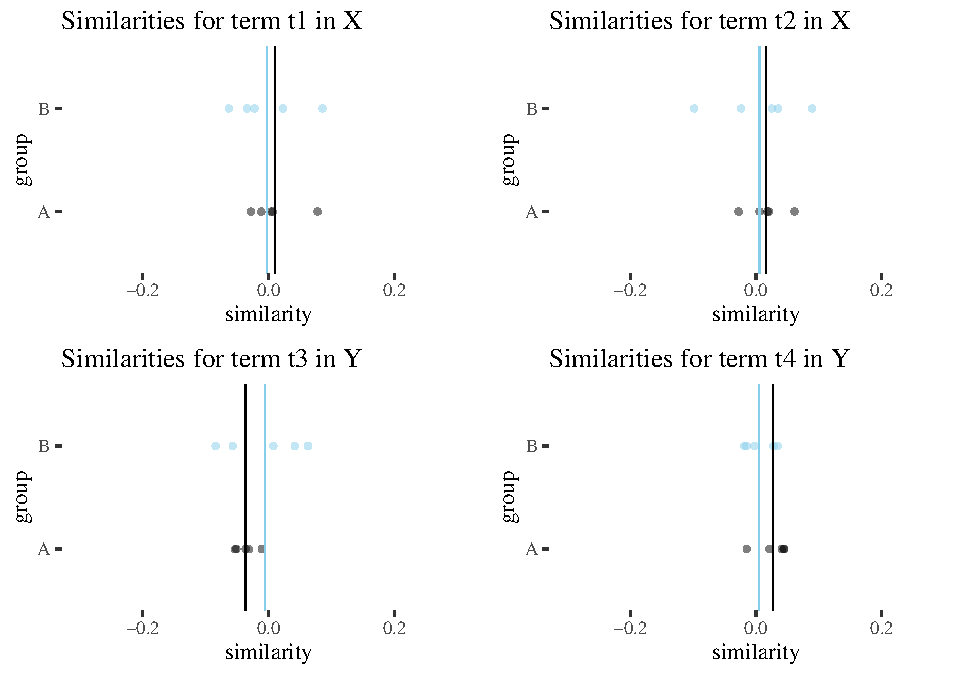
\includegraphics[width=1\linewidth]{paperDraft_files/figure-latex/unnamed-chunk-2-1} \end{center}

\noindent When you look at the datapoints, do you have the impression of
a strong bias here? We wouldn't think so. But now let's run the
calculations from (Caliskan et al., 2017).

\vspace{1mm} \footnotesize

\begin{Shaded}
\begin{Highlighting}[]
\NormalTok{s <-}\StringTok{ }\ControlFlowTok{function}\NormalTok{ (table)\{ }\KeywordTok{mean}\NormalTok{(table}\OperatorTok{$}\NormalTok{A) }\OperatorTok{-}\StringTok{ }\KeywordTok{mean}\NormalTok{(table}\OperatorTok{$}\NormalTok{B)\}}
\NormalTok{factor <-}\StringTok{ }\KeywordTok{sd}\NormalTok{(}\KeywordTok{c}\NormalTok{(}\KeywordTok{s}\NormalTok{(t1),}\KeywordTok{s}\NormalTok{(t2),}\KeywordTok{s}\NormalTok{(t3),}\KeywordTok{s}\NormalTok{(t4)))}
\NormalTok{numerator <-}\StringTok{  }\KeywordTok{mean}\NormalTok{(}\KeywordTok{s}\NormalTok{(t1),}\KeywordTok{s}\NormalTok{(t2)) }\OperatorTok{-}\StringTok{ }\KeywordTok{mean}\NormalTok{(}\KeywordTok{s}\NormalTok{(t3),}\KeywordTok{s}\NormalTok{(t4))}
\KeywordTok{print}\NormalTok{(}\KeywordTok{list}\NormalTok{(}\DataTypeTok{factor =}\NormalTok{ factor,}\DataTypeTok{numerator =}\NormalTok{ numerator, }\DataTypeTok{bias =}\NormalTok{ numerator }\OperatorTok{/}\StringTok{ }\NormalTok{factor))}
\end{Highlighting}
\end{Shaded}

\begin{verbatim}
## $factor
## [1] 0.02342637
## 
## $numerator
## [1] 0.04275325
## 
## $bias
## [1] 1.825005
\end{verbatim}

\normalsize

\noindent This should make us pause. We know these were points randomly
drawn from distributions where there is no difference in means. Yet, the
calculated effect size is 1.82, whereas the largest effect size reported
by Caliskan et al. (2017) is 1.81!

Interestingly, if we repeat the drawing 10000 times, each time
calculating the bias, it turns out that with this variance and sample
size, pretty much anything can happen.

\vspace{1mm} \footnotesize

\begin{Shaded}
\begin{Highlighting}[]
\NormalTok{biasesNull <-}\StringTok{ }\KeywordTok{numeric}\NormalTok{(}\DecValTok{10000}\NormalTok{)}
\ControlFlowTok{for}\NormalTok{(i }\ControlFlowTok{in} \DecValTok{1}\OperatorTok{:}\DecValTok{10000}\NormalTok{)\{}
\NormalTok{t1 <-}\StringTok{ }\KeywordTok{data.frame}\NormalTok{(}\DataTypeTok{A  =} \KeywordTok{rnorm}\NormalTok{(}\DecValTok{5}\NormalTok{,}\DecValTok{0}\NormalTok{,}\FloatTok{0.05}\NormalTok{), }\DataTypeTok{B =} \KeywordTok{rnorm}\NormalTok{(}\DecValTok{5}\NormalTok{,}\DecValTok{0}\NormalTok{,}\FloatTok{0.05}\NormalTok{))}
\NormalTok{t2 <-}\StringTok{ }\KeywordTok{data.frame}\NormalTok{(}\DataTypeTok{A  =} \KeywordTok{rnorm}\NormalTok{(}\DecValTok{5}\NormalTok{,}\DecValTok{0}\NormalTok{,}\FloatTok{0.05}\NormalTok{), }\DataTypeTok{B =} \KeywordTok{rnorm}\NormalTok{(}\DecValTok{5}\NormalTok{,}\DecValTok{0}\NormalTok{,}\FloatTok{0.05}\NormalTok{))}
\NormalTok{t3 <-}\StringTok{ }\KeywordTok{data.frame}\NormalTok{(}\DataTypeTok{A  =} \KeywordTok{rnorm}\NormalTok{(}\DecValTok{5}\NormalTok{,}\DecValTok{0}\NormalTok{,}\FloatTok{0.05}\NormalTok{), }\DataTypeTok{B =} \KeywordTok{rnorm}\NormalTok{(}\DecValTok{5}\NormalTok{,}\DecValTok{0}\NormalTok{,}\FloatTok{0.05}\NormalTok{))}
\NormalTok{t4 <-}\StringTok{ }\KeywordTok{data.frame}\NormalTok{(}\DataTypeTok{A  =} \KeywordTok{rnorm}\NormalTok{(}\DecValTok{5}\NormalTok{,}\DecValTok{0}\NormalTok{,}\FloatTok{0.05}\NormalTok{), }\DataTypeTok{B =} \KeywordTok{rnorm}\NormalTok{(}\DecValTok{5}\NormalTok{,}\DecValTok{0}\NormalTok{,}\FloatTok{0.05}\NormalTok{))}

\NormalTok{factor <-}\StringTok{ }\KeywordTok{sd}\NormalTok{(}\KeywordTok{c}\NormalTok{(}\KeywordTok{s}\NormalTok{(t1),}\KeywordTok{s}\NormalTok{(t2),}\KeywordTok{s}\NormalTok{(t3),}\KeywordTok{s}\NormalTok{(t4)))}
\NormalTok{numerator <-}\StringTok{  }\KeywordTok{mean}\NormalTok{(}\KeywordTok{s}\NormalTok{(t1),}\KeywordTok{s}\NormalTok{(t2)) }\OperatorTok{-}\StringTok{ }\KeywordTok{mean}\NormalTok{(}\KeywordTok{s}\NormalTok{(t3),}\KeywordTok{s}\NormalTok{(t4))}
\NormalTok{biasesNull[i]  <-}\StringTok{ }\NormalTok{numerator }\OperatorTok{/}\StringTok{ }\NormalTok{factor}
\NormalTok{\}}
\KeywordTok{ggplot}\NormalTok{()}\OperatorTok{+}\KeywordTok{geom_histogram}\NormalTok{(}\KeywordTok{aes}\NormalTok{(}\DataTypeTok{x=}\NormalTok{biasesNull, }\DataTypeTok{y =}\NormalTok{ ..density..), }\DataTypeTok{alpha =} \FloatTok{0.6}\NormalTok{, }\DataTypeTok{bins=}\DecValTok{50}\NormalTok{)}\OperatorTok{+}
\StringTok{  }\KeywordTok{theme_tufte}\NormalTok{()}\OperatorTok{+}\KeywordTok{labs}\NormalTok{(}\DataTypeTok{title=}\StringTok{"10k biases for identical means and sd =.05"}\NormalTok{)}\OperatorTok{+}\StringTok{ }\KeywordTok{xlab}\NormalTok{(}\StringTok{"bias"}\NormalTok{)}
\end{Highlighting}
\end{Shaded}

\begin{center}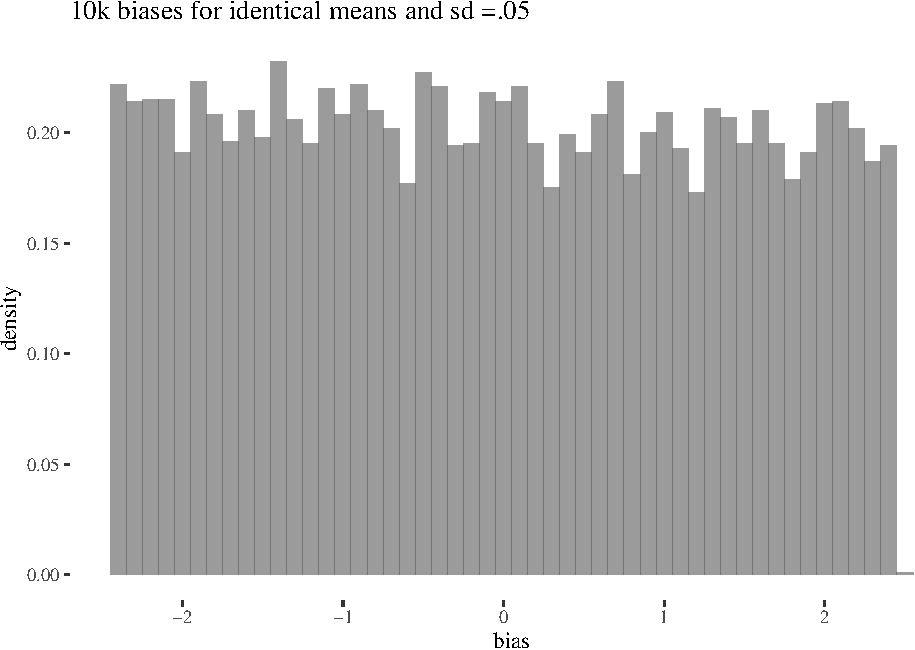
\includegraphics[width=1\linewidth]{paperDraft_files/figure-latex/unnamed-chunk-4-1} \end{center}

\normalsize

Now, let's simulate a situation where the means are identical but the
standard deviation is much smaller, .001.

\footnotesize

\begin{Shaded}
\begin{Highlighting}[]
\KeywordTok{set.seed}\NormalTok{(}\DecValTok{124}\NormalTok{)}
\NormalTok{t1v <-}\StringTok{ }\KeywordTok{data.frame}\NormalTok{(}\DataTypeTok{A  =} \KeywordTok{rnorm}\NormalTok{(}\DecValTok{5}\NormalTok{,}\DecValTok{0}\NormalTok{,}\FloatTok{0.001}\NormalTok{), }\DataTypeTok{B =} \KeywordTok{rnorm}\NormalTok{(}\DecValTok{5}\NormalTok{,}\DecValTok{0}\NormalTok{,}\FloatTok{0.001}\NormalTok{))}
\NormalTok{t2v <-}\StringTok{ }\KeywordTok{data.frame}\NormalTok{(}\DataTypeTok{A  =} \KeywordTok{rnorm}\NormalTok{(}\DecValTok{5}\NormalTok{,}\DecValTok{0}\NormalTok{,}\FloatTok{0.001}\NormalTok{), }\DataTypeTok{B =} \KeywordTok{rnorm}\NormalTok{(}\DecValTok{5}\NormalTok{,}\DecValTok{0}\NormalTok{,}\FloatTok{0.001}\NormalTok{))}
\NormalTok{t3v <-}\StringTok{ }\KeywordTok{data.frame}\NormalTok{(}\DataTypeTok{A  =} \KeywordTok{rnorm}\NormalTok{(}\DecValTok{5}\NormalTok{,}\DecValTok{0}\NormalTok{,}\FloatTok{0.001}\NormalTok{), }\DataTypeTok{B =} \KeywordTok{rnorm}\NormalTok{(}\DecValTok{5}\NormalTok{,}\DecValTok{0}\NormalTok{,}\FloatTok{0.001}\NormalTok{))}
\NormalTok{t4v <-}\StringTok{ }\KeywordTok{data.frame}\NormalTok{(}\DataTypeTok{A  =} \KeywordTok{rnorm}\NormalTok{(}\DecValTok{5}\NormalTok{,}\DecValTok{0}\NormalTok{,}\FloatTok{0.001}\NormalTok{), }\DataTypeTok{B =} \KeywordTok{rnorm}\NormalTok{(}\DecValTok{5}\NormalTok{,}\DecValTok{0}\NormalTok{,}\FloatTok{0.001}\NormalTok{))}
\end{Highlighting}
\end{Shaded}

\normalsize

\begin{center}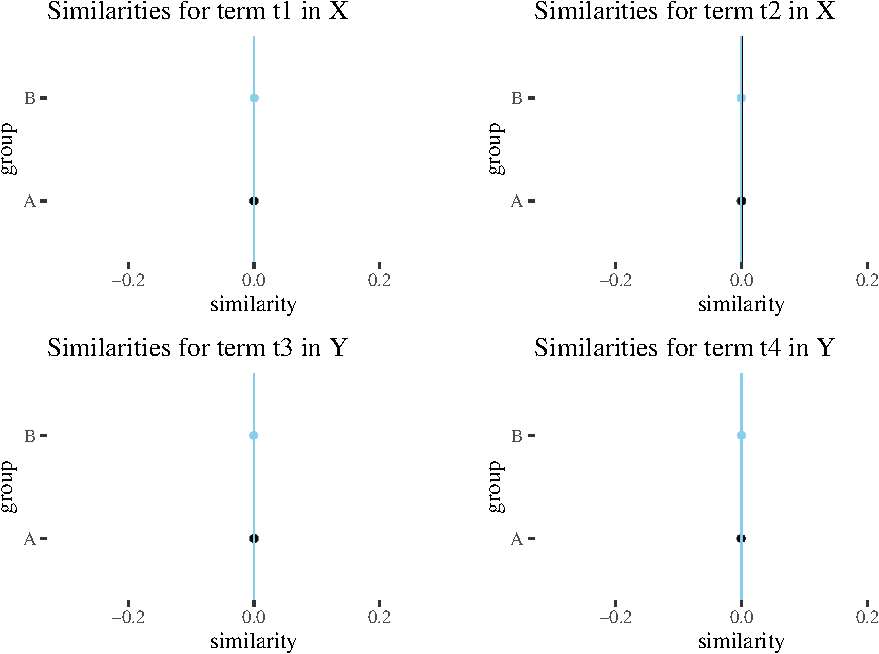
\includegraphics[width=1\linewidth]{paperDraft_files/figure-latex/unnamed-chunk-6-1} \end{center}

\noindent When you look at the datapoints, do you have the impression of
a strong bias here? We wouldn't think so. But now let's run the
calculations from (Caliskan et al., 2017).

\vspace{1mm} \footnotesize

\begin{Shaded}
\begin{Highlighting}[]
\NormalTok{factorV <-}\StringTok{ }\KeywordTok{sd}\NormalTok{(}\KeywordTok{c}\NormalTok{(}\KeywordTok{s}\NormalTok{(t1v),}\KeywordTok{s}\NormalTok{(t2v),}\KeywordTok{s}\NormalTok{(t3v),}\KeywordTok{s}\NormalTok{(t4v)))}
\NormalTok{numeratorV <-}\StringTok{  }\KeywordTok{mean}\NormalTok{(}\KeywordTok{s}\NormalTok{(t1v),}\KeywordTok{s}\NormalTok{(t2v)) }\OperatorTok{-}\StringTok{ }\KeywordTok{mean}\NormalTok{(}\KeywordTok{s}\NormalTok{(t3v),}\KeywordTok{s}\NormalTok{(t4v))}
\KeywordTok{print}\NormalTok{(}\KeywordTok{list}\NormalTok{(}\DataTypeTok{factor =}\NormalTok{ factorV,}\DataTypeTok{numerator =}\NormalTok{ numeratorV, }\DataTypeTok{bias =}\NormalTok{ numeratorV }\OperatorTok{/}\StringTok{ }\NormalTok{factorV))}
\end{Highlighting}
\end{Shaded}

\begin{verbatim}
## $factor
## [1] 0.0006402666
## 
## $numerator
## [1] -0.001237637
## 
## $bias
## [1] -1.933003
\end{verbatim}

\normalsize

While the numerator and the factors changed a lot, the bias actually
increased. One reason bias increases is that once the standard deviation
goes down, so does the factor used in the calculation of bias.

Again, to see whether this metric would provide us with meaningful
information, let's simulate 10000 drawings.

\vspace{1mm} \footnotesize

\begin{Shaded}
\begin{Highlighting}[]
\KeywordTok{set.seed}\NormalTok{(}\DecValTok{124}\NormalTok{)}

\NormalTok{biasesLowVariance <-}\StringTok{ }\KeywordTok{numeric}\NormalTok{(}\DecValTok{10000}\NormalTok{)}
\ControlFlowTok{for}\NormalTok{(i }\ControlFlowTok{in} \DecValTok{1}\OperatorTok{:}\DecValTok{10000}\NormalTok{)\{}
\NormalTok{t1v <-}\StringTok{ }\KeywordTok{data.frame}\NormalTok{(}\DataTypeTok{A  =} \KeywordTok{rnorm}\NormalTok{(}\DecValTok{5}\NormalTok{,}\DecValTok{0}\NormalTok{,}\FloatTok{0.001}\NormalTok{), }\DataTypeTok{B =} \KeywordTok{rnorm}\NormalTok{(}\DecValTok{5}\NormalTok{,}\DecValTok{0}\NormalTok{,}\FloatTok{0.001}\NormalTok{))}
\NormalTok{t2v <-}\StringTok{ }\KeywordTok{data.frame}\NormalTok{(}\DataTypeTok{A  =} \KeywordTok{rnorm}\NormalTok{(}\DecValTok{5}\NormalTok{,}\DecValTok{0}\NormalTok{,}\FloatTok{0.001}\NormalTok{), }\DataTypeTok{B =} \KeywordTok{rnorm}\NormalTok{(}\DecValTok{5}\NormalTok{,}\DecValTok{0}\NormalTok{,}\FloatTok{0.001}\NormalTok{))}
\NormalTok{t3v <-}\StringTok{ }\KeywordTok{data.frame}\NormalTok{(}\DataTypeTok{A  =} \KeywordTok{rnorm}\NormalTok{(}\DecValTok{5}\NormalTok{,}\DecValTok{0}\NormalTok{,}\FloatTok{0.001}\NormalTok{), }\DataTypeTok{B =} \KeywordTok{rnorm}\NormalTok{(}\DecValTok{5}\NormalTok{,}\DecValTok{0}\NormalTok{,}\FloatTok{0.001}\NormalTok{))}
\NormalTok{t4v <-}\StringTok{ }\KeywordTok{data.frame}\NormalTok{(}\DataTypeTok{A  =} \KeywordTok{rnorm}\NormalTok{(}\DecValTok{5}\NormalTok{,}\DecValTok{0}\NormalTok{,}\FloatTok{0.001}\NormalTok{), }\DataTypeTok{B =} \KeywordTok{rnorm}\NormalTok{(}\DecValTok{5}\NormalTok{,}\DecValTok{0}\NormalTok{,}\FloatTok{0.001}\NormalTok{))}

\NormalTok{factorV <-}\StringTok{ }\KeywordTok{sd}\NormalTok{(}\KeywordTok{c}\NormalTok{(}\KeywordTok{s}\NormalTok{(t1v),}\KeywordTok{s}\NormalTok{(t2v),}\KeywordTok{s}\NormalTok{(t3v),}\KeywordTok{s}\NormalTok{(t4v)))}

\NormalTok{numeratorV <-}\StringTok{  }\KeywordTok{mean}\NormalTok{(}\KeywordTok{s}\NormalTok{(t1v),}\KeywordTok{s}\NormalTok{(t2v)) }\OperatorTok{-}\StringTok{ }\KeywordTok{mean}\NormalTok{(}\KeywordTok{s}\NormalTok{(t3v),}\KeywordTok{s}\NormalTok{(t4v))}

\NormalTok{biasesLowVariance[i] <-}\StringTok{ }\NormalTok{numeratorV }\OperatorTok{/}\StringTok{ }\NormalTok{factorV}
\NormalTok{\}}
\KeywordTok{ggplot}\NormalTok{()}\OperatorTok{+}\KeywordTok{geom_histogram}\NormalTok{(}\KeywordTok{aes}\NormalTok{(}\DataTypeTok{x=}\NormalTok{biasesLowVariance, }\DataTypeTok{y =}\NormalTok{ ..density..), }\DataTypeTok{alpha =} \FloatTok{0.6}\NormalTok{, }\DataTypeTok{bins=}\DecValTok{50}\NormalTok{)}\OperatorTok{+}
\StringTok{  }\KeywordTok{theme_tufte}\NormalTok{()}\OperatorTok{+}\KeywordTok{labs}\NormalTok{(}\DataTypeTok{title=}\StringTok{"10k biases for identical means and sd =.001"}\NormalTok{)}\OperatorTok{+}\StringTok{ }\KeywordTok{xlab}\NormalTok{(}\StringTok{"bias"}\NormalTok{)}
\end{Highlighting}
\end{Shaded}

\begin{center}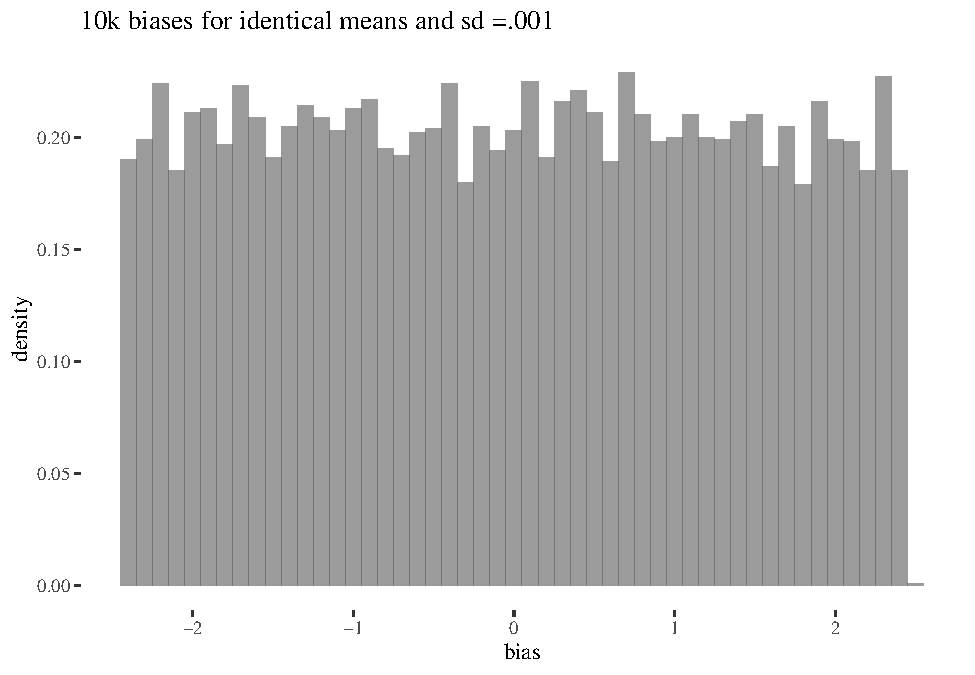
\includegraphics[width=1\linewidth]{paperDraft_files/figure-latex/unnamed-chunk-8-1} \end{center}

\normalsize

Again, not so informative. Now, let's try sampling from distributions
where there in fact is a difference in means. Terms from \(X\) are on
average .1 similar to \(A\) (and still \(0\) to \(B\)), while terms from
\(Y\) are \(.1\) similar to \(B\) (and 0 to \(A\)). The standard
deviation is 0.05 in all the cases. There is a clear difference between
\(X\) and \(Y\) and quick visual inspection should tell us so.

\vspace{1mm} \footnotesize

\begin{Shaded}
\begin{Highlighting}[]
\KeywordTok{set.seed}\NormalTok{(}\DecValTok{766}\NormalTok{)}
\NormalTok{t1d2 <-}\StringTok{ }\KeywordTok{data.frame}\NormalTok{(}\DataTypeTok{A  =} \KeywordTok{rnorm}\NormalTok{(}\DecValTok{5}\NormalTok{,.}\DecValTok{1}\NormalTok{,}\FloatTok{0.05}\NormalTok{), }\DataTypeTok{B =} \KeywordTok{rnorm}\NormalTok{(}\DecValTok{5}\NormalTok{,}\DecValTok{0}\NormalTok{,}\FloatTok{0.05}\NormalTok{))}
\NormalTok{t2d2 <-}\StringTok{ }\KeywordTok{data.frame}\NormalTok{(}\DataTypeTok{A  =} \KeywordTok{rnorm}\NormalTok{(}\DecValTok{5}\NormalTok{,.}\DecValTok{1}\NormalTok{,}\FloatTok{0.05}\NormalTok{), }\DataTypeTok{B =} \KeywordTok{rnorm}\NormalTok{(}\DecValTok{5}\NormalTok{,}\DecValTok{0}\NormalTok{,}\FloatTok{0.05}\NormalTok{))}
\NormalTok{t3d2 <-}\StringTok{ }\KeywordTok{data.frame}\NormalTok{(}\DataTypeTok{A  =} \KeywordTok{rnorm}\NormalTok{(}\DecValTok{5}\NormalTok{,}\DecValTok{0}\NormalTok{,}\FloatTok{0.05}\NormalTok{), }\DataTypeTok{B =} \KeywordTok{rnorm}\NormalTok{(}\DecValTok{5}\NormalTok{,.}\DecValTok{1}\NormalTok{,}\FloatTok{0.05}\NormalTok{))}
\NormalTok{t4d2 <-}\StringTok{ }\KeywordTok{data.frame}\NormalTok{(}\DataTypeTok{A  =} \KeywordTok{rnorm}\NormalTok{(}\DecValTok{5}\NormalTok{,}\DecValTok{0}\NormalTok{,}\FloatTok{0.05}\NormalTok{), }\DataTypeTok{B =} \KeywordTok{rnorm}\NormalTok{(}\DecValTok{5}\NormalTok{,.}\DecValTok{1}\NormalTok{,}\FloatTok{0.05}\NormalTok{))}
\end{Highlighting}
\end{Shaded}

\normalsize

\vspace{1mm} \footnotesize

\begin{center}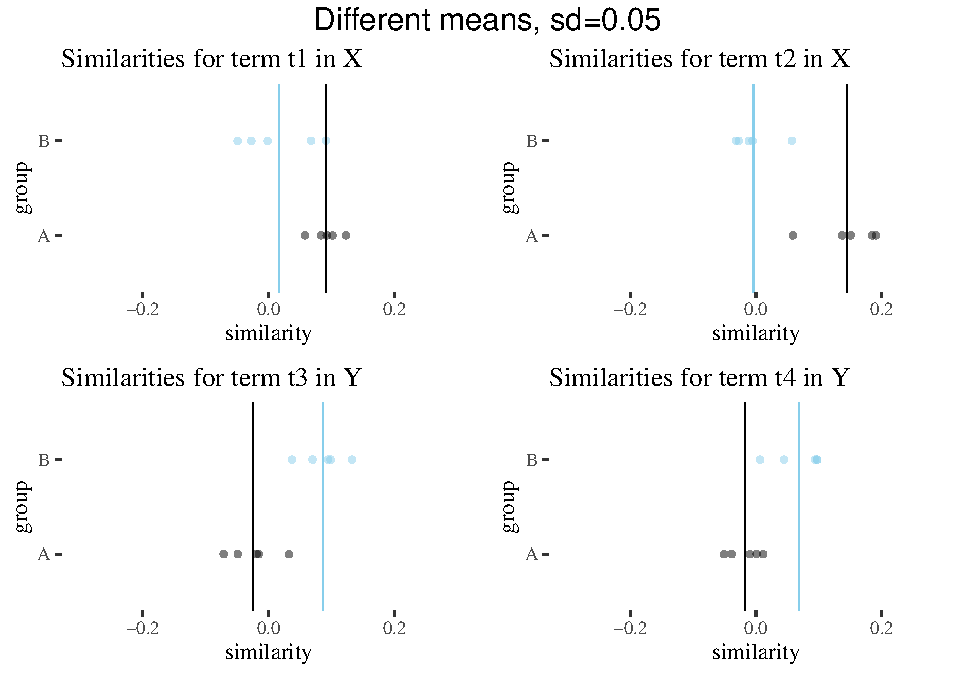
\includegraphics[width=1\linewidth]{paperDraft_files/figure-latex/unnamed-chunk-10-1} \end{center}

\normalsize

\noindent  Is this clear difference mirrored in the calculations?

\footnotesize

\begin{Shaded}
\begin{Highlighting}[]
\NormalTok{factorD2 <-}\StringTok{ }\KeywordTok{sd}\NormalTok{(}\KeywordTok{c}\NormalTok{(}\KeywordTok{s}\NormalTok{(t1d2),}\KeywordTok{s}\NormalTok{(t2d2),}\KeywordTok{s}\NormalTok{(t3d2),}\KeywordTok{s}\NormalTok{(t4d2)))}
\NormalTok{numeratorD2 <-}\StringTok{  }\KeywordTok{mean}\NormalTok{(}\KeywordTok{s}\NormalTok{(t1d2),}\KeywordTok{s}\NormalTok{(t2d2)) }\OperatorTok{-}\StringTok{ }\KeywordTok{mean}\NormalTok{(}\KeywordTok{s}\NormalTok{(t3d2),}\KeywordTok{s}\NormalTok{(t4d2))}
\NormalTok{biasD2 <-}\StringTok{ }\NormalTok{numeratorD2 }\OperatorTok{/}\StringTok{ }\NormalTok{factorD2}
\NormalTok{biasD2}
\end{Highlighting}
\end{Shaded}

\begin{verbatim}
## [1] 1.490014
\end{verbatim}

\normalsize 

\noindent The absolute value of the effect size is smaller than in the
null case with the same standard deviation. Let's simulate 10000
drawings:

\vspace{1mm} \footnotesize

\begin{Shaded}
\begin{Highlighting}[]
\NormalTok{biasesD2 <-}\StringTok{ }\KeywordTok{numeric}\NormalTok{(}\DecValTok{10000}\NormalTok{)}
\ControlFlowTok{for}\NormalTok{(i }\ControlFlowTok{in} \DecValTok{1}\OperatorTok{:}\DecValTok{10000}\NormalTok{)\{}
\NormalTok{t1d2 <-}\StringTok{ }\KeywordTok{data.frame}\NormalTok{(}\DataTypeTok{A  =} \KeywordTok{rnorm}\NormalTok{(}\DecValTok{5}\NormalTok{,.}\DecValTok{1}\NormalTok{,}\FloatTok{0.05}\NormalTok{), }\DataTypeTok{B =} \KeywordTok{rnorm}\NormalTok{(}\DecValTok{5}\NormalTok{,}\DecValTok{0}\NormalTok{,}\FloatTok{0.05}\NormalTok{))}
\NormalTok{t2d2 <-}\StringTok{ }\KeywordTok{data.frame}\NormalTok{(}\DataTypeTok{A  =} \KeywordTok{rnorm}\NormalTok{(}\DecValTok{5}\NormalTok{,.}\DecValTok{1}\NormalTok{,}\FloatTok{0.05}\NormalTok{), }\DataTypeTok{B =} \KeywordTok{rnorm}\NormalTok{(}\DecValTok{5}\NormalTok{,}\DecValTok{0}\NormalTok{,}\FloatTok{0.05}\NormalTok{))}
\NormalTok{t3d2 <-}\StringTok{ }\KeywordTok{data.frame}\NormalTok{(}\DataTypeTok{A  =} \KeywordTok{rnorm}\NormalTok{(}\DecValTok{5}\NormalTok{,}\DecValTok{0}\NormalTok{,}\FloatTok{0.05}\NormalTok{), }\DataTypeTok{B =} \KeywordTok{rnorm}\NormalTok{(}\DecValTok{5}\NormalTok{,.}\DecValTok{1}\NormalTok{,}\FloatTok{0.05}\NormalTok{))}
\NormalTok{t4d2 <-}\StringTok{ }\KeywordTok{data.frame}\NormalTok{(}\DataTypeTok{A  =} \KeywordTok{rnorm}\NormalTok{(}\DecValTok{5}\NormalTok{,}\DecValTok{0}\NormalTok{,}\FloatTok{0.05}\NormalTok{), }\DataTypeTok{B =} \KeywordTok{rnorm}\NormalTok{(}\DecValTok{5}\NormalTok{,.}\DecValTok{1}\NormalTok{,}\FloatTok{0.05}\NormalTok{))}

\NormalTok{factorD2 <-}\StringTok{ }\KeywordTok{sd}\NormalTok{(}\KeywordTok{c}\NormalTok{(}\KeywordTok{s}\NormalTok{(t1d2),}\KeywordTok{s}\NormalTok{(t2d2),}\KeywordTok{s}\NormalTok{(t3d2),}\KeywordTok{s}\NormalTok{(t4d2)))}
\NormalTok{numeratorD2 <-}\StringTok{  }\KeywordTok{mean}\NormalTok{(}\KeywordTok{s}\NormalTok{(t1d2),}\KeywordTok{s}\NormalTok{(t2d2)) }\OperatorTok{-}\StringTok{ }\KeywordTok{mean}\NormalTok{(}\KeywordTok{s}\NormalTok{(t3d2),}\KeywordTok{s}\NormalTok{(t4d2))}
\NormalTok{biasesD2[i] <-}\StringTok{ }\NormalTok{numeratorD2}\OperatorTok{/}\NormalTok{factorD2}
\NormalTok{\}}

\KeywordTok{ggplot}\NormalTok{()}\OperatorTok{+}\KeywordTok{geom_histogram}\NormalTok{(}\KeywordTok{aes}\NormalTok{(}\DataTypeTok{x=}\NormalTok{biasesD2, }\DataTypeTok{y =}\NormalTok{ ..density..), }\DataTypeTok{alpha =} \FloatTok{0.6}\NormalTok{, }\DataTypeTok{bins=}\DecValTok{50}\NormalTok{)}\OperatorTok{+}
\StringTok{  }\KeywordTok{theme_tufte}\NormalTok{()}\OperatorTok{+}\KeywordTok{labs}\NormalTok{(}\DataTypeTok{title=}\StringTok{"10k biases for different means and sd =.05"}\NormalTok{)}\OperatorTok{+}\StringTok{ }\KeywordTok{xlab}\NormalTok{(}\StringTok{"bias"}\NormalTok{)}
\end{Highlighting}
\end{Shaded}

\begin{center}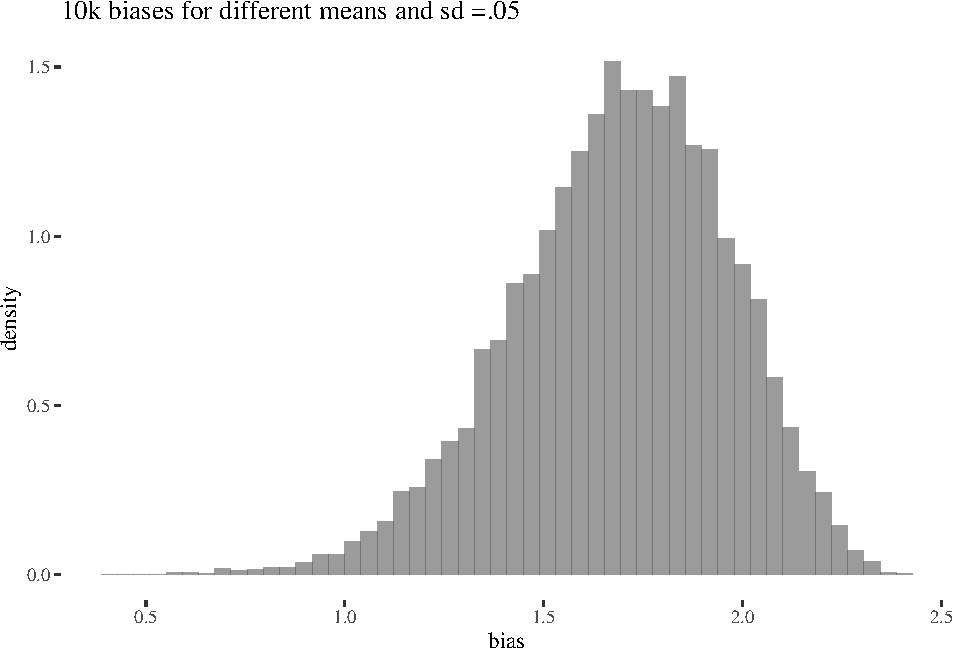
\includegraphics[width=1\linewidth]{paperDraft_files/figure-latex/unnamed-chunk-12-1} \end{center}

\normalsize

\noindent Now suppose we keep the means the same but increase the
standard deviation to .1.

\vspace{1mm} \footnotesize

\begin{Shaded}
\begin{Highlighting}[]
\KeywordTok{set.seed}\NormalTok{(}\DecValTok{766}\NormalTok{)}
\NormalTok{t1d1 <-}\StringTok{ }\KeywordTok{data.frame}\NormalTok{(}\DataTypeTok{A  =} \KeywordTok{rnorm}\NormalTok{(}\DecValTok{5}\NormalTok{,.}\DecValTok{1}\NormalTok{,}\FloatTok{0.1}\NormalTok{), }\DataTypeTok{B =} \KeywordTok{rnorm}\NormalTok{(}\DecValTok{5}\NormalTok{,}\DecValTok{0}\NormalTok{,}\FloatTok{0.1}\NormalTok{))}
\NormalTok{t2d1 <-}\StringTok{ }\KeywordTok{data.frame}\NormalTok{(}\DataTypeTok{A  =} \KeywordTok{rnorm}\NormalTok{(}\DecValTok{5}\NormalTok{,.}\DecValTok{1}\NormalTok{,}\FloatTok{0.1}\NormalTok{), }\DataTypeTok{B =} \KeywordTok{rnorm}\NormalTok{(}\DecValTok{5}\NormalTok{,}\DecValTok{0}\NormalTok{,}\FloatTok{0.1}\NormalTok{))}
\NormalTok{t3d1 <-}\StringTok{ }\KeywordTok{data.frame}\NormalTok{(}\DataTypeTok{A  =} \KeywordTok{rnorm}\NormalTok{(}\DecValTok{5}\NormalTok{,}\DecValTok{0}\NormalTok{,}\FloatTok{0.1}\NormalTok{), }\DataTypeTok{B =} \KeywordTok{rnorm}\NormalTok{(}\DecValTok{5}\NormalTok{,.}\DecValTok{1}\NormalTok{,}\FloatTok{0.1}\NormalTok{))}
\NormalTok{t4d1 <-}\StringTok{ }\KeywordTok{data.frame}\NormalTok{(}\DataTypeTok{A  =} \KeywordTok{rnorm}\NormalTok{(}\DecValTok{5}\NormalTok{,}\DecValTok{0}\NormalTok{,}\FloatTok{0.1}\NormalTok{), }\DataTypeTok{B =} \KeywordTok{rnorm}\NormalTok{(}\DecValTok{5}\NormalTok{,.}\DecValTok{1}\NormalTok{,}\FloatTok{0.1}\NormalTok{))}
\end{Highlighting}
\end{Shaded}

\normalsize

\vspace{1mm} \footnotesize

\begin{center}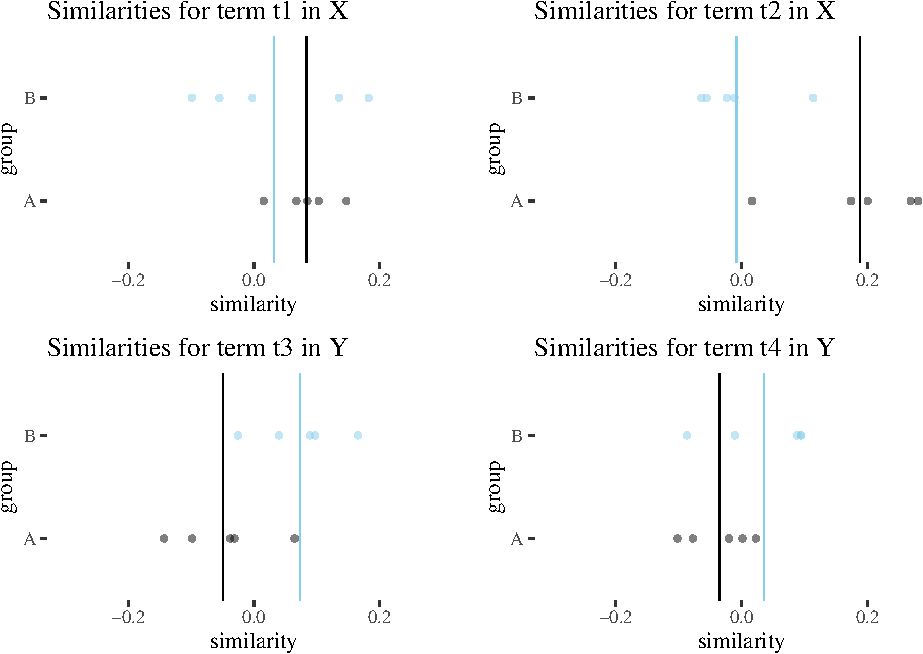
\includegraphics[width=1\linewidth]{paperDraft_files/figure-latex/unnamed-chunk-14-1} \end{center}

\normalsize

\noindent  Is this clear difference mirrored in the calculations?

\footnotesize

\begin{Shaded}
\begin{Highlighting}[]
\NormalTok{factorD1 <-}\StringTok{ }\KeywordTok{sd}\NormalTok{(}\KeywordTok{c}\NormalTok{(}\KeywordTok{s}\NormalTok{(t1d1),}\KeywordTok{s}\NormalTok{(t2d1),}\KeywordTok{s}\NormalTok{(t3d1),}\KeywordTok{s}\NormalTok{(t4d1)))}
\NormalTok{numeratorD1 <-}\StringTok{  }\KeywordTok{mean}\NormalTok{(}\KeywordTok{s}\NormalTok{(t1d1),}\KeywordTok{s}\NormalTok{(t2d1)) }\OperatorTok{-}\StringTok{ }\KeywordTok{mean}\NormalTok{(}\KeywordTok{s}\NormalTok{(t3d1),}\KeywordTok{s}\NormalTok{(t4d1))}
\NormalTok{biasD1 <-}\StringTok{ }\NormalTok{numeratorD1 }\OperatorTok{/}\StringTok{ }\NormalTok{factorD1}
\NormalTok{biasD1}
\end{Highlighting}
\end{Shaded}

\begin{verbatim}
## [1] 1.223023
\end{verbatim}

\normalsize 

\noindent The absolute value of the effect size is smaller than in the
previous case!

\vspace{1mm} \footnotesize

\begin{Shaded}
\begin{Highlighting}[]
\NormalTok{biasesD1 <-}\StringTok{ }\KeywordTok{numeric}\NormalTok{(}\DecValTok{10000}\NormalTok{)}

\ControlFlowTok{for}\NormalTok{(i }\ControlFlowTok{in} \DecValTok{1}\OperatorTok{:}\DecValTok{10000}\NormalTok{)\{}
\NormalTok{t1d1 <-}\StringTok{ }\KeywordTok{data.frame}\NormalTok{(}\DataTypeTok{A  =} \KeywordTok{rnorm}\NormalTok{(}\DecValTok{5}\NormalTok{,.}\DecValTok{1}\NormalTok{,}\FloatTok{0.1}\NormalTok{), }\DataTypeTok{B =} \KeywordTok{rnorm}\NormalTok{(}\DecValTok{5}\NormalTok{,}\DecValTok{0}\NormalTok{,}\FloatTok{0.1}\NormalTok{))}
\NormalTok{t2d1 <-}\StringTok{ }\KeywordTok{data.frame}\NormalTok{(}\DataTypeTok{A  =} \KeywordTok{rnorm}\NormalTok{(}\DecValTok{5}\NormalTok{,.}\DecValTok{1}\NormalTok{,}\FloatTok{0.1}\NormalTok{), }\DataTypeTok{B =} \KeywordTok{rnorm}\NormalTok{(}\DecValTok{5}\NormalTok{,}\DecValTok{0}\NormalTok{,}\FloatTok{0.1}\NormalTok{))}
\NormalTok{t3d1 <-}\StringTok{ }\KeywordTok{data.frame}\NormalTok{(}\DataTypeTok{A  =} \KeywordTok{rnorm}\NormalTok{(}\DecValTok{5}\NormalTok{,}\DecValTok{0}\NormalTok{,}\FloatTok{0.1}\NormalTok{), }\DataTypeTok{B =} \KeywordTok{rnorm}\NormalTok{(}\DecValTok{5}\NormalTok{,.}\DecValTok{1}\NormalTok{,}\FloatTok{0.1}\NormalTok{))}
\NormalTok{t4d1 <-}\StringTok{ }\KeywordTok{data.frame}\NormalTok{(}\DataTypeTok{A  =} \KeywordTok{rnorm}\NormalTok{(}\DecValTok{5}\NormalTok{,}\DecValTok{0}\NormalTok{,}\FloatTok{0.1}\NormalTok{), }\DataTypeTok{B =} \KeywordTok{rnorm}\NormalTok{(}\DecValTok{5}\NormalTok{,.}\DecValTok{1}\NormalTok{,}\FloatTok{0.1}\NormalTok{))}

\NormalTok{factorD1 <-}\StringTok{ }\KeywordTok{sd}\NormalTok{(}\KeywordTok{c}\NormalTok{(}\KeywordTok{s}\NormalTok{(t1d1),}\KeywordTok{s}\NormalTok{(t2d1),}\KeywordTok{s}\NormalTok{(t3d1),}\KeywordTok{s}\NormalTok{(t4d1)))}
\NormalTok{numeratorD1 <-}\StringTok{  }\KeywordTok{mean}\NormalTok{(}\KeywordTok{s}\NormalTok{(t1d1),}\KeywordTok{s}\NormalTok{(t2d1)) }\OperatorTok{-}\StringTok{ }\KeywordTok{mean}\NormalTok{(}\KeywordTok{s}\NormalTok{(t3d1),}\KeywordTok{s}\NormalTok{(t4d1))}
\NormalTok{biasesD1[i] <-}\StringTok{ }\NormalTok{numeratorD1}\OperatorTok{/}\NormalTok{factorD1}
\NormalTok{\}}

\KeywordTok{ggplot}\NormalTok{()}\OperatorTok{+}\KeywordTok{geom_histogram}\NormalTok{(}\KeywordTok{aes}\NormalTok{(}\DataTypeTok{x=}\NormalTok{biasesD1, }\DataTypeTok{y =}\NormalTok{ ..density..), }\DataTypeTok{alpha =} \FloatTok{0.6}\NormalTok{, }\DataTypeTok{bins=}\DecValTok{50}\NormalTok{)}\OperatorTok{+}
\StringTok{  }\KeywordTok{theme_tufte}\NormalTok{()}\OperatorTok{+}\KeywordTok{labs}\NormalTok{(}\DataTypeTok{title=}\StringTok{"10k biases for different means and sd =.001"}\NormalTok{)}\OperatorTok{+}\StringTok{ }\KeywordTok{xlab}\NormalTok{(}\StringTok{"bias"}\NormalTok{)}
\end{Highlighting}
\end{Shaded}

\begin{center}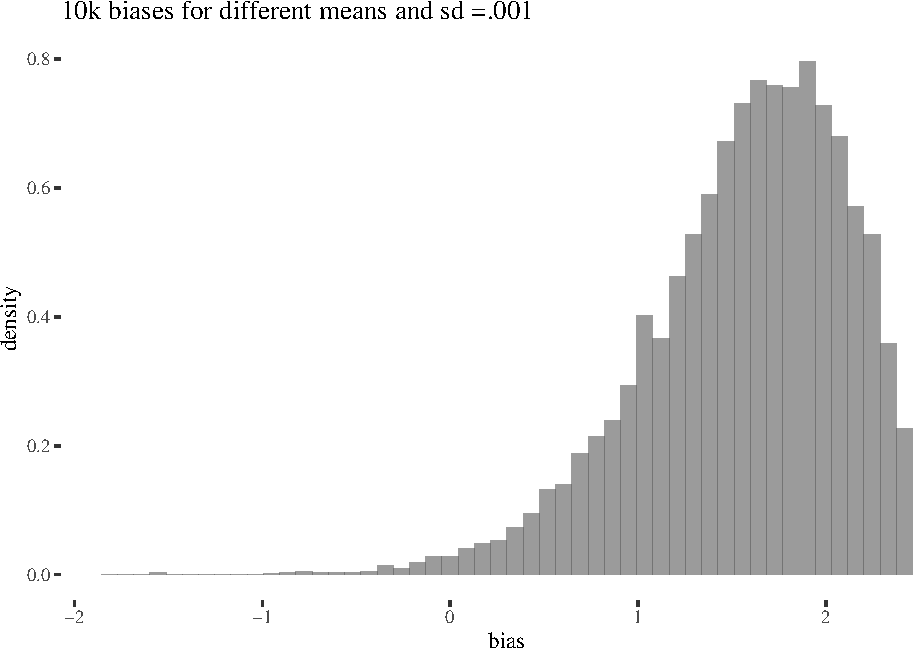
\includegraphics[width=1\linewidth]{paperDraft_files/figure-latex/unnamed-chunk-16-1} \end{center}

\normalsize

This is is a bit better, but still quite some uncertainty is involved,
far from what systematically low mean-based p-values reported in the
papers might suggest. Of course, this is a bit of a caricature, as our
word lists were short (four protected words and 10 attributes). But the
word lists used in the actually papers are not much longer. In such a
set-up the key observations are as follows:

\begin{itemize}
\item
  Seemingly high bias measures might arise even if the underlying
  processes actually have the same mean.
\item
  Even if the mean remains the same, non-negligible changes can result
  from a shift in the standard deviation of the original process, and
  the change might go in the opposite direction than a visualisation of
  datapoints might suggest, because with the decrease of standard
  deviation, the factor decreases and the bias increases.
\item
  Even if the underlying means are the same, but the variation is
  different, the bias metric in the long run could tend toward a
  different value:
\item
  The lack of control group in the paper and our analysis indicates that
  without neutral baseline it is difficult to interpret the
  effectiveness of the metric.
\end{itemize}

\vspace{1mm} \footnotesize

\begin{Shaded}
\begin{Highlighting}[]
\KeywordTok{mean}\NormalTok{(biasesD1); }\KeywordTok{mean}\NormalTok{(biasesD2)}
\end{Highlighting}
\end{Shaded}

\begin{verbatim}
## [1] 1.563319
\end{verbatim}

\begin{verbatim}
## [1] 1.690664
\end{verbatim}

\begin{Shaded}
\begin{Highlighting}[]
\KeywordTok{median}\NormalTok{(biasesD1); }\KeywordTok{median}\NormalTok{(biasesD2)}
\end{Highlighting}
\end{Shaded}

\begin{verbatim}
## [1] 1.638136
\end{verbatim}

\begin{verbatim}
## [1] 1.707511
\end{verbatim}

\normalsize
and so the point estimations of bias are sensitive to factors other than
the underlying process means.

\begin{itemize}
\item
  Even if there is a difference in means, the bias metric can be lower,
  and the uncertainty about it needs to be gauged.
\item
  The uncertainty resulting from including the raw datapoint variance
  into considerations is more extensive than the one suggested by the
  low p-values obtained from taking means as datapoints.
\end{itemize}

\vspace{1mm} \footnotesize

\begin{Shaded}
\begin{Highlighting}[]
\KeywordTok{quantile}\NormalTok{(biasesD2, }\DataTypeTok{probs =} \KeywordTok{c}\NormalTok{(}\FloatTok{0.275}\NormalTok{,}\FloatTok{0.975}\NormalTok{))}
\end{Highlighting}
\end{Shaded}

\begin{verbatim}
##    27.5%    97.5% 
## 1.539149 2.166488
\end{verbatim}

\begin{Shaded}
\begin{Highlighting}[]
\KeywordTok{quantile}\NormalTok{(biasesD1, }\DataTypeTok{probs =} \KeywordTok{c}\NormalTok{(}\FloatTok{0.275}\NormalTok{,}\FloatTok{0.975}\NormalTok{))}
\end{Highlighting}
\end{Shaded}

\begin{verbatim}
##    27.5%    97.5% 
## 1.300648 2.356815
\end{verbatim}

\normalsize

\section{Bayesian estimation}\label{bayesian-estimation}

\begin{itemize}
\item
  reddit i google, ogolnie i z podzialem na protected words
\item
  dokladniej gender, reszta na koniec w zalaczniku
\end{itemize}

\section{Effects of debiasing}\label{effects-of-debiasing}

\section{Discussion}\label{discussion}

\newpage

\noindent \huge  \textbf{Appendix} \normalsize

\noindent \Large \textbf{Word lists, including human and neutral predicates}
\normalsize

\section*{References}\label{references}
\addcontentsline{toc}{section}{References}

\vspace{-3mm}

\hypertarget{refs}{}
\hypertarget{ref-bolukbasi2016man}{}
Bolukbasi, T., Chang, K.-W., Zou, J., Saligrama, V., \& Kalai, A.
(2016). Man is to computer programmer as woman is to homemaker?
Debiasing word embeddings.

\hypertarget{ref-Caliskan2017semanticsBiases}{}
Caliskan, A., Bryson, J. J., \& Narayanan, A. (2017). Semantics derived
automatically from language corpora contain human-like biases.
\emph{Science}, \emph{356}(6334), 183--186. American Association for the
Advancement of Science (AAAS). Retrieved from
\url{https://doi.org/10.1126/science.aal4230}

\hypertarget{ref-Garg2018years}{}
Garg, N., Schiebinger, L., Jurafsky, D., \& Zou, J. (2018). Word
embeddings quantify 100 years of gender and ethnic stereotypes.
\emph{Proceedings of the National Academy of Sciences}, \emph{115}(16),
E3635--E3644. Proceedings of the National Academy of Sciences. Retrieved
from \url{https://doi.org/10.1073/pnas.1720347115}

\hypertarget{ref-Gonen2019lipstick}{}
Gonen, H., \& Goldberg, Y. (2019). Lipstick on a pig: Debiasing methods
cover up systematic gender biases in word embeddings but do not remove
them. In \emph{Proceedings of the 2019 conference of the north American
chapter of the association for computational linguistics: Human language
technologies, volume 1 (long and short papers)} (pp. 609--614).
Minneapolis, Minnesota: Association for Computational Linguistics.
Retrieved from \url{https://www.aclweb.org/anthology/N19-1061}

\hypertarget{ref-Lauscher2019multidimensional}{}
Lauscher, A., \& Glavas, G. (2019). Are we consistently biased?
Multidimensional analysis of biases in distributional word vectors.
\emph{CoRR}, \emph{abs/1904.11783}. Retrieved from
\url{http://arxiv.org/abs/1904.11783}

\hypertarget{ref-Nissim2020fair}{}
Nissim, M., Noord, R. van, \& Goot, R. van der. (2020). Fair is better
than sensational: Man is to doctor as woman is to doctor.
\emph{Computational Linguistics}, \emph{46}(2), 487--497. MIT Press -
Journals. Retrieved from \url{https://doi.org/10.1162/coli_a_00379}

\hypertarget{ref-Nosek2002harvesting}{}
Nosek, B. A., Banaji, M. R., \& Greenwald, A. G. (2002). Harvesting
implicit group attitudes and beliefs from a demonstration web site.
\emph{Group Dynamics: Theory, Research, and Practice}, \emph{6}(1),
101--115. American Psychological Association (APA). Retrieved from
\url{https://doi.org/10.1037/1089-2699.6.1.101}

\end{document}
